\section{Introduction}

\subsection{Motivation}
The renewed focus on robotic exploration of the lunar surface presents distinct challenges for autonomous navigation~\cite{eurocons}. Long-range traverses are required in environments characterized by poorly textured regolith, high-contrast shadows, and the absence of atmospheric scattering. Furthermore, rovers are often limited to radiation-hardened computing hardware and vision-based sensors, precluding the use of active sensors like LiDAR. These constraints necessitate the development of computationally efficient, vision-based mapping and localization solutions.

Simultaneous Localization and Mapping (SLAM) is a standard approach for building a map of an unknown environment while tracking an agent's position within it. Classical SLAM methods, such as those based on geometric features, can operate in real time but exhibit reduced performance in the texture-deficient and high-contrast lighting conditions common on the Moon. While learning-based SLAM methods can improve robustness by learning feature representations from data, their generalization to novel environments like the lunar surface is not guaranteed. A common limitation of both classical and early learning-based methods is their reliance on discrete map representations (e.g., point clouds, voxels), which can be memory-intensive and may not capture fine surface detail.

\subsection{Related Work}

Recent advances in neural scene representations have produced methods capable of high-fidelity 3D reconstruction from images. A recent survey~\cite{tosi_how_2024} details the rapid evolution of this field for terrestrial applications, covering approaches that use various sensor modalities (e.g., monocular, stereo, depth, IMU) and scene encodings (e.g., Neural Radiance Fields (NeRF), 3D Gaussian Splatting (3DGS), neural point clouds). These systems often rely on perception models for tasks like feature extraction, depth estimation, or semantic understanding. However, since these perception components are typically trained on terrestrial data, it is not clear whether their performance will generalize to the unique visual characteristics of extraterrestrial environments.

Semantic understanding of planetary environments is an active area of research. A systematic literature review on semantic terrain segmentation for planetary rovers~\cite{kuang_semantic_2022} highlights a gap in existing solutions, noting that no current method simultaneously achieves pixel-level accuracy, real-time inference, and compatibility with onboard hardware. Specific models have shown promise for feature identification, such as detecting impact craters from digital elevation models~\cite{jia_moon_2021}. Despite these advances in perception, the integration of such semantic information into modern neural mapping frameworks for planetary surfaces has not been thoroughly investigated.

Several works have applied neural scene representations to model the lunar surface. Some have focused on surface reconstruction from orbital imagery to generate digital elevation models, often to handle challenging illumination in permanently shadowed regions~\cite{van_kints_neural_2025, adams_summary_2023}. More relevant to rover navigation, a few recent studies have explored using NeRFs with surface-level imagery for localization, mapping, and path planning~\cite{huang_monocular_2025, hansen_analyzing_2024, dai_neural_2023, zhang_neural_2024}. These approaches demonstrate the potential of neural representations for capturing lunar terrain.

However, existing works for surface mapping predominantly rely on NeRF~\cite{mildenhall_nerf_2021}, which has several limitations for real-time, incremental rover navigation. First, NeRF's rendering process is computationally expensive due to its reliance on volumetric sampling, making it ill-suited for real-time applications on resource-constrained hardware. Second, the underlying multi-layer perceptron (MLP) represents a fixed volume, which is difficult to extend as the rover explores new areas and is not easily deformable to accommodate loop closures. This necessitates stitching multiple models, which can introduce inconsistencies. Finally, the implicit nature of NeRF makes it less interpretable and difficult to integrate with or query for explicit semantic information. Many of these works also assume diverse camera viewpoints during training, a condition not met by the typically forward-facing trajectory of a rover.

\subsection{Contributions}
This work addresses the aforementioned limitations by developing a framework for building semantically-aware, large-scale maps of the lunar surface in real time. Our primary contributions are:
\begin{itemize}
	\item We propose a real-time mapping framework for lunar surface environments based on 3D Gaussian Splatting, which offers fast rendering and a flexible, explicit scene representation suitable for incremental updates.
	\item We integrate and benchmark a suite of dense perception models, including semantic segmentation and both stereo and monocular depth estimation networks adapted for lunar conditions. We analyze the direct impact of these perception inputs on the geometric and semantic quality of the final 3D reconstruction.
\end{itemize}


\subsection{Paper Organization}
The rest of the paper is organized as follows.


\begin{figure}[b]
	\centering
	\begin{subfigure}[b]{0.55\linewidth}
		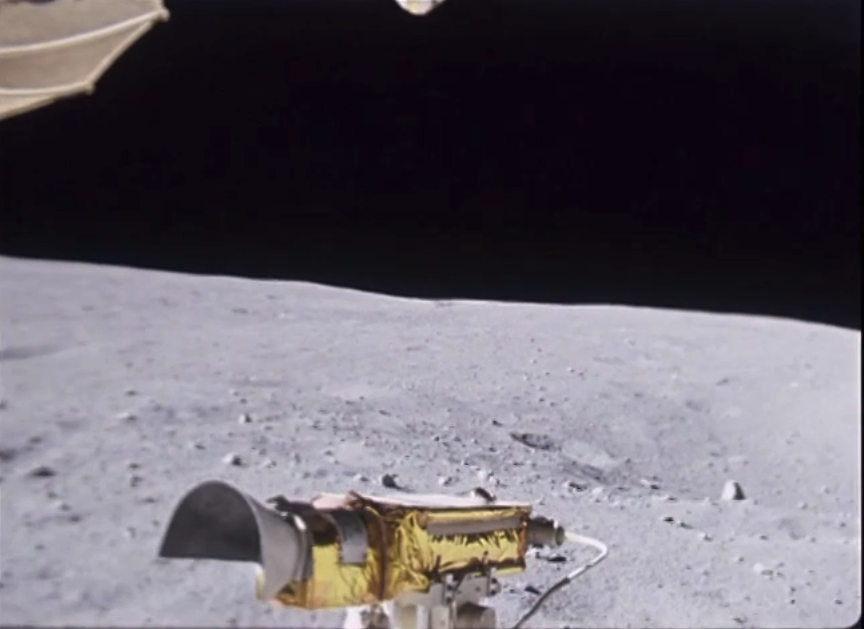
\includegraphics[width=\linewidth,trim=0 0.5 0.5em 0,clip]{figures/rover2.png}
	\end{subfigure}
	\begin{subfigure}[b]{0.395\linewidth}
		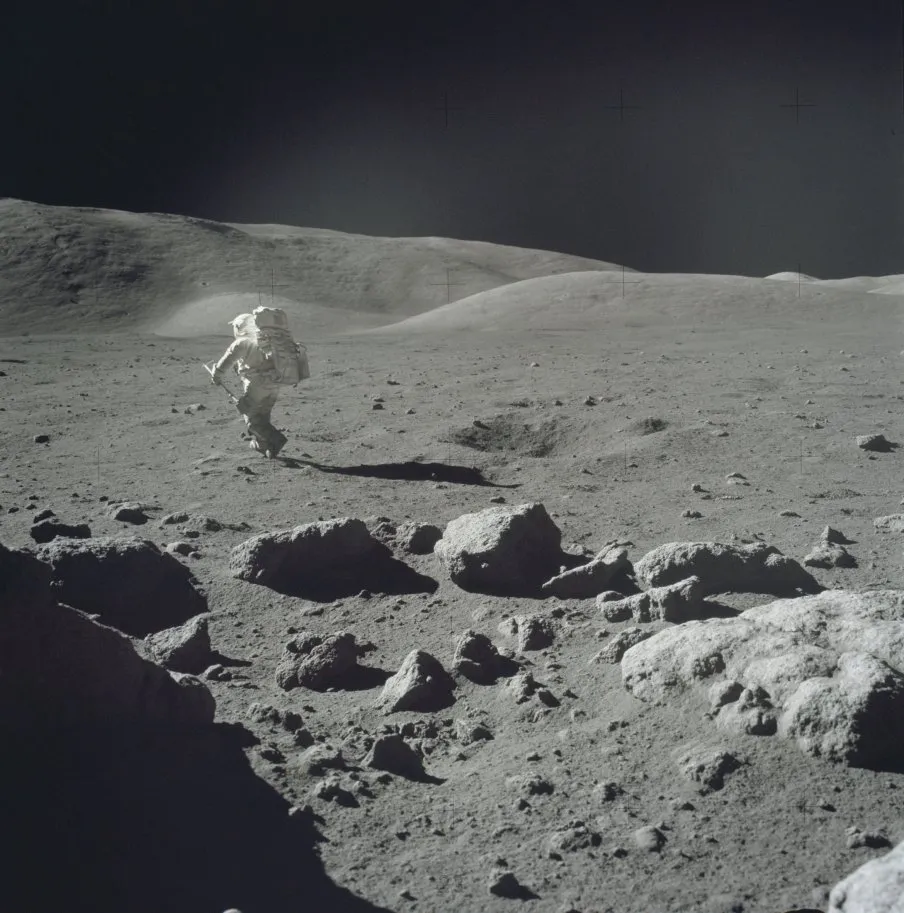
\includegraphics[width=\linewidth,trim=0 0.5 0.5em 0,clip]{figures/surface_astronaut.png}
	\end{subfigure}
	\caption{\bfseries Images from the Apollo missions~\cite{nasa_apollo_2017}.}
\end{figure}

% \begin{figure*}[t]
% 	\centering
% 	% \begin{subfigure}[t]{0.33\linewidth}
% 	%   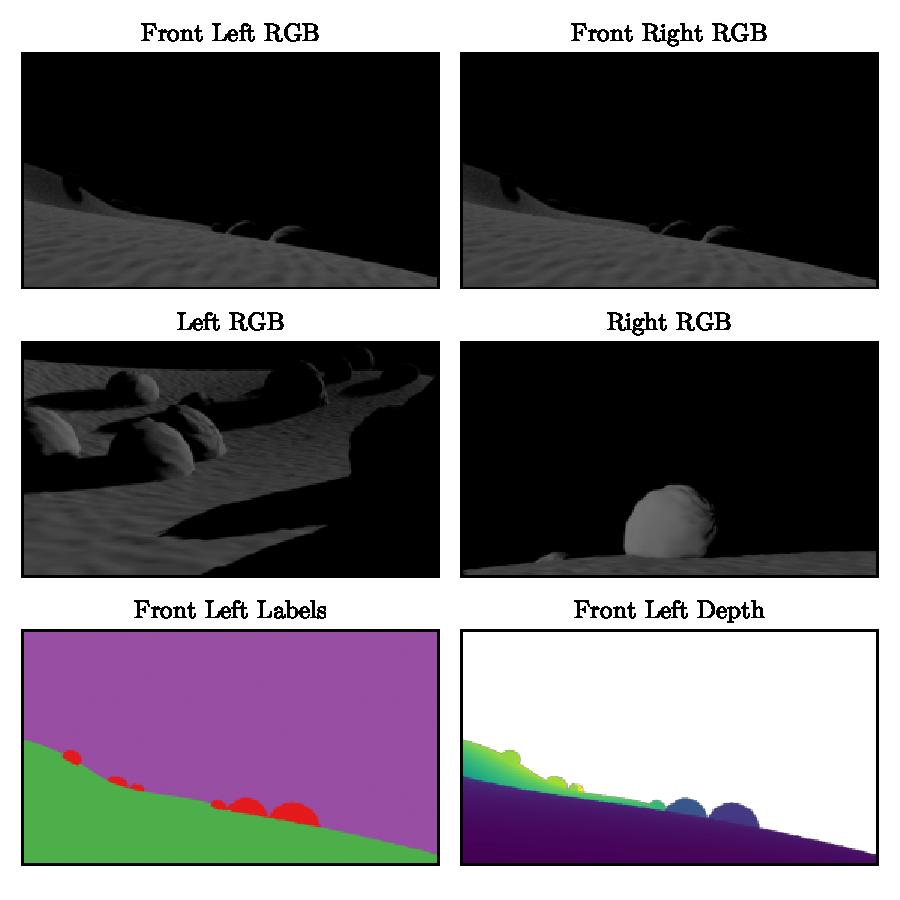
\includegraphics[width=\linewidth]{figures/sample_open3d.pdf}
% 	%   \caption{\bfseries Open3D environment.}
% 	%   \label{fig:sample_open3d}
% 	% \end{subfigure}
% 	\begin{subfigure}[t]{0.33\linewidth}
% 		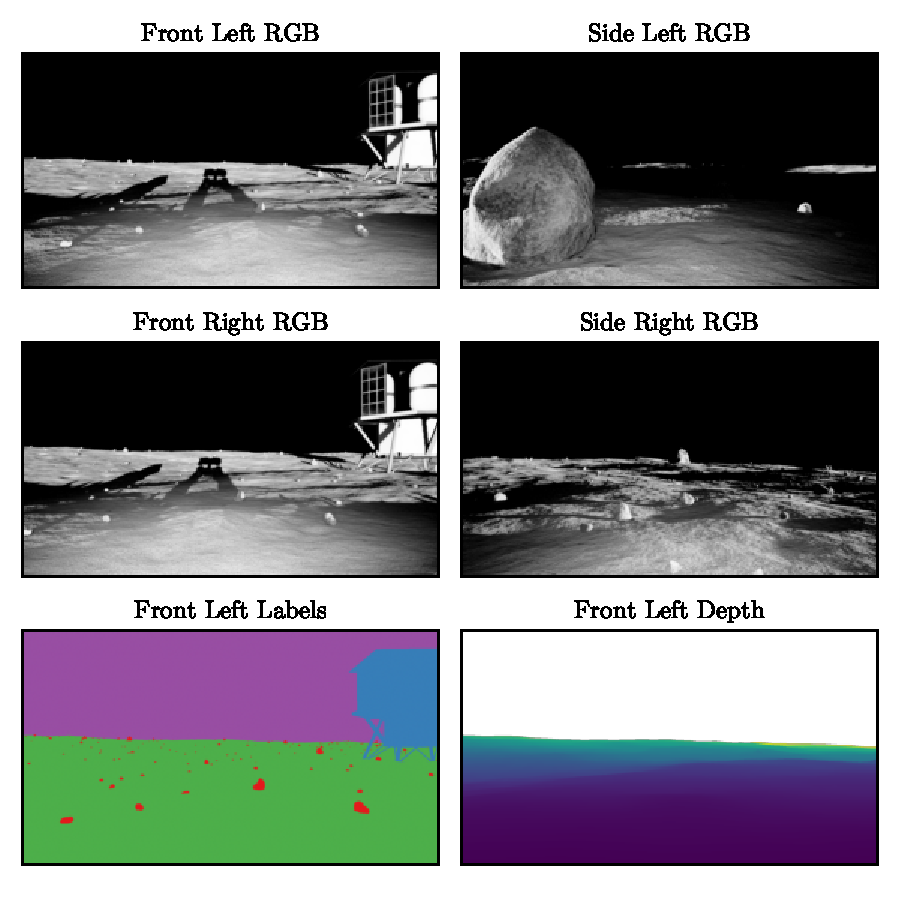
\includegraphics[width=\linewidth]{figures/sample_lac.pdf}
% 		\caption{\bfseries LAC environment.}\label{fig:sample_lac}
% 	\end{subfigure}
% 	\begin{subfigure}[t]{0.33\linewidth}
% 		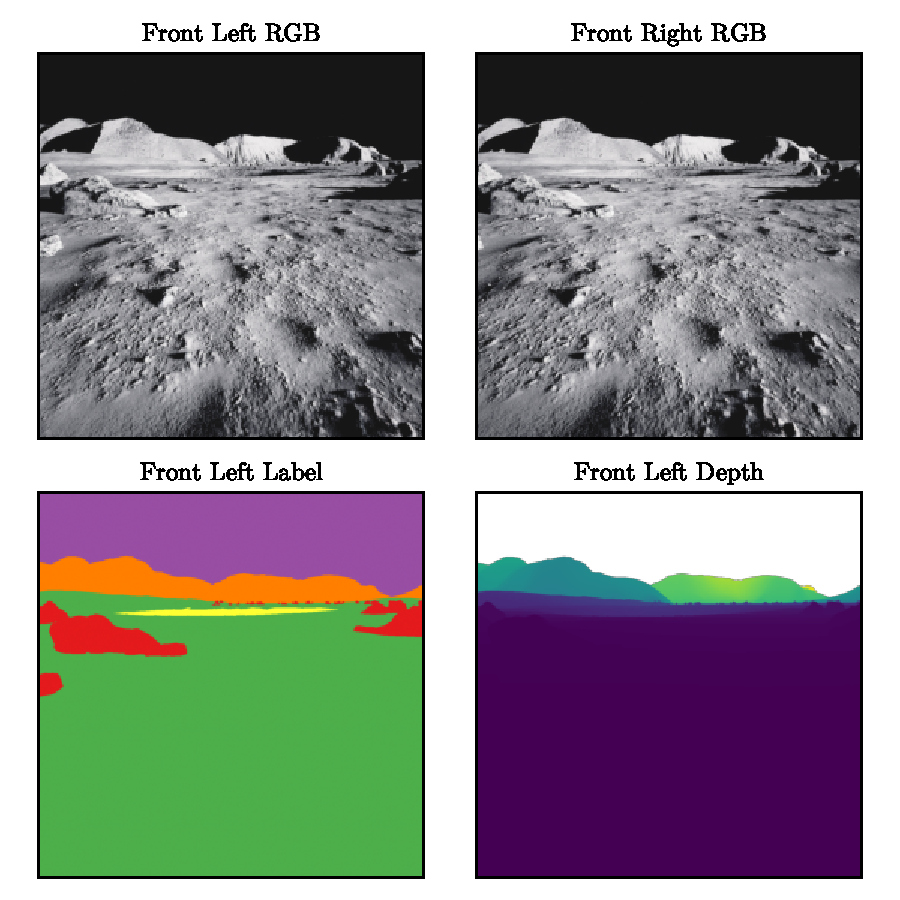
\includegraphics[width=\linewidth]{figures/sample_lusnar.pdf}
% 		\caption{\bfseries LuSNAR dataset.}\label{fig:sample_lusnar}
% 	\end{subfigure}
% 	\caption{\bfseries Sample images from different environments.}\label{fig:sample_environments}
% \end{figure*}

\begin{figure}[t]
	\centering
	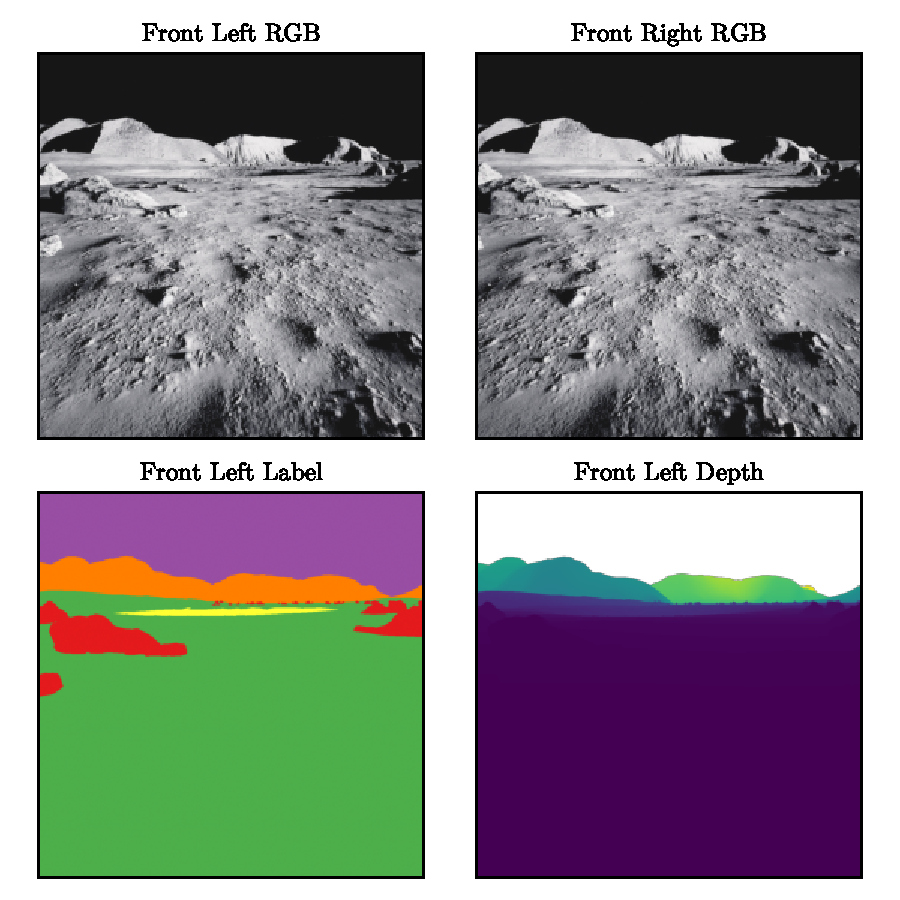
\includegraphics[width=\linewidth]{figures/sample_lusnar.pdf}
	\caption{\bfseries Sample images from the LuSNAR dataset.}
	\label{fig:sample_lusnar}
\end{figure}

As traverse speeds increase, real-time perception becomes even more critical for safe autonomous navigation. Accurate dense depth estimation and semantic segmentation are essential for precise distance measurements to hazards, untraversable terrain, and shadowed regions where obstacles may be hidden. These complementary modalities provide the geometric and semantic understanding of the scene necessary for safe and efficient navigation.
In this work, we propose a real-time 3D Gaussian splatting framework for mapping that leverages both depth estimation and semantic segmentation models adapted for lunar environments. Our approach focuses on improving the performance of these vision-based perception modules under challenging lunar conditions, enabling robust real-time mapping using neural scene representations.
